\documentclass{report}
\usepackage{caption}
\usepackage{subcaption}
\usepackage[T1]{fontenc}
\usepackage[utf8]{inputenc}
\usepackage{import}
\usepackage[english]{babel}
\usepackage{amssymb}
\usepackage{minted}
\usepackage{tikz}
\usepackage{amsthm}
\usepackage{amsmath}
\usepackage{graphicx}

\usepackage{biblatex}
\usepackage{longtable}
\usepackage{csquotes}
\usepackage[poorman]{cleveref}
\usepackage{tabularray}
\addbibresource{bbl.bib}
\newtheorem{theorem}{Theorem}
\newtheorem{definition}{Definition}
\newtheorem{remark}{Remark}
\newtheorem{notation}{Notation}
\newtheorem{invariant}{Invariant}

\begin{document}
\begin{titlepage}
	\begin{center}
        
		\large
		\textbf{Jagiellonian University}\\
		Department of Theoretical Computer Science\\

		\vspace{1.5cm}

		\Large
		\textbf{Artur Salawa}

		\vspace*{2cm}

		\textbf{\LARGE Implementation of exponential algorithms for the independent set  problem}
		
		\vspace{0.5cm}
		\large
		
		\vfill
		\Large
		Bachelor's Thesis

		\vfill
		\Large
		Supervisor: dr hab. in\.z. Krzysztof Turowski
		
		\vspace{0.8cm}
		
		August 2023
		
\end{center}
\end{titlepage}

\pagebreak
\tableofcontents

\pagebreak


\chapter{Definitions}
\section{Definitions}

We first give some basic definitions in graph theory sourced from~\cite{bollobás1998modern}.

\begin{defn}[graph]
    A \emph{graph} $G$ is an ordered pair of disjoint sets $(V, E)$ such that $E$ is a subset of the set $V \choose 2$ of unordered pairs of $V$. 
\end{defn}

We only consider finite graphs, that is, $V$ and $E$ are always finite. The set $V$ is the set of \emph{vertices} and $E$ is the set of \emph{edges}. If $G$ is a graph, then $V = V(G)$ is the \emph{vertex set} of $G$, and $E = E(G)$ is the \emph{edge set} of $G$. If $v$ is a vertex of $G$ we will sometimes write $v \in G$ instead of $v \in V(G)$. 

We denote $n_G = |V(G)|$ and $m_G = |E(G)|$ for a graph $G = (V, E)$. We will drop the subscripts for brevity when $G$ is clear from the context.

An edge $\{ x, y \}$ is said to \emph{join} the vertices $x$ and $y$ and is denoted $xy$. Thus, $xy$ and $yx$ mean exactly the same edge, the vertices $x$ and $y$ are the \emph{endvertices} of this edge. If $xy \in E(G)$, then $x$ and $y$ are \emph{adjacent}, \emph{neighboring} or \emph{connected}, and the  vertices $x$ and $y$ are \emph{incident} with the edge $xy$. Two edges are \emph{adjacent} if the have exactly one common endvertex.

The set of vertices adjacent to a vertex $v \in G$.

\begin{defn}[subgraph]
    We say that $G' = (V', E')$ is a \emph{subgraph} of $G = (V, E)$ if $V' \subseteq V$ and $E' \subseteq E$. In this case we write $G' \subseteq G$. If $G'$ contains all edges of $G$ that join two vertices in $V'$ then $G'$ is said to be a subgraph \emph{induced} or \emph{spanned} by $B'$ and is denoted $G[V']$. 
\end{defn}

For a subgraph $G' = G[H]$ spanned by a vertex subset $H \subseteq V(G)$, we write $n_H = |H|$ and $m_H = |E(G')|$.

If $W \subseteq V(G)$, then $G - W = G[V \setminus W]$ is the subgraph of $G$ obtained by deleting the vertices of $W$ and all edges incident with them. Similarly, if $E' \subseteq E(G)$, then $G - E' = (V(G), E(G) \setminus E')$. If $W = \{ w \}$ and $E' = \{ xy \}$ for some vertex $w \in V(G)$ and edge $xy \in E(G)$, then the notation is simplified to $G - w$ and $G - xy$. Similarly, if $x$ and $y$ are nonadjacent vertices of $G$, then $G + xy = (V(G), E(G) \cup \{ xy \})$.

\begin{defn}[path]
    A \emph{path} is a graph $P$ of the form

    \begin{align*}
        V(P) &= \{x_0, x_1, \dots, x_l\} \\
        E(P) &= \{x_0x_1, x_1x_2, \dots, x_{l-1}x_l\}
    \end{align*}
\end{defn}

This path $P$ is usually denoted by $x_0x_1\dots x_l$. The vertices $x_0$ and $x_l$ are the \emph{ends} of $P$ and the value $l = |E(P)|$ is the \emph{length} of $P$. We say that $P$ goes from $x_0$ to $x_l$.

\begin{defn}[connected graph]
    A graph is \emph{connected} if for every pair $\{x, y\}$ of distinct vertices there is a path from $x$ to $y$.
\end{defn}

A maximal connected subgraph is a \emph{component} of a graph.

\begin{defn}[cycle]
    A \emph{cycle} is a graph $C$ of the form

    \begin{align*}
        V(C) &= \{x_0, x_1, \dots, x_l\} \\
        E(C) &= \{x_0x_1, x_1x_2, \dots, x_{l-1}x_l, x_l x_0\}
    \end{align*}
\end{defn}

This cycle $C$ is denoted by $x_0 x_1\dots x_l x_1$. The value $l + 1 = |E(C)| = |V(C)|$ is the \emph{length} of $C$. 

\begin{defn}[forest, tree]
    A graph without any cycles is a \emph{forest}, or an \emph{acyclic} graph. A \emph{tree} is connected forest.
\end{defn}

\begin{defn}[bipartite graph]
    A graph $G$ is a \emph{bipartite} graph with vertex classes $V_1$ and $V_2$ if $V(G) = V_1 \cup V_2$, $V_1 \cap V_2 = \emptyset$ and every edge joins a vertex of $V_1$ to a vertex of $V_2$.
\end{defn}

An easy observation is that a graph is bipartite if and only if it does not contain an odd-length cycle.

A set of vertices (edges) is \emph{independent} if no two elements of it are adjacent.

\begin{defn}[matching]
    A set of independent edges is called a \emph{matching}. A matching $M$ is \emph{perfect} if every vertex is adjacent to exactly one edge in $M$.
\end{defn}

\begin{defn}[exposed vertices]
    A vertex $v$ is \emph{exposed} for a matching $M$ if it is not adjacent to any edge in $M$. If a vertex is not exposed it is \emph{matched}.
\end{defn}

If a vertex $v$ is matched in a matching $M$, then we call the vertex $u$, such that $uv \in M$, the \emph{mate} or \emph{matched vertex} of $v$ and the edge $\{u, v\}$ the \emph{matched edge} of $v$.

\begin{defn}[alternating path]
    A path $P = x_0x_1\dots x_l$ is alternating for a matching $M$ if for each $i \in \{0, \dots, l - 2\}$, $x_i x_{i+1} \in M$ if and only if $x_{i+1}x_{i+2} \notin M$.
\end{defn}

\begin{defn}[augmenting path]
    An alternating path $x_0x_1\dots x_l$ is \emph{augmenting} if the vertices $x_0$ and $x_l$ are both exposed.
\end{defn}

\begin{defn}[weighted graph]
    A \emph{weighted} graph is a graph $G = (V, E)$ along with a \emph{weight function} $w : E \rightarrow \mathbb{R}$, which assigns a real valued \emph{weight} $w(e)$ to each edge of $G$.
\end{defn}

For a set of edges $S \subseteq E$, we define the \emph{weight} of $S$ to be $w(S) = \sum_{e \in S} w(e)$. 

We denote $N_G = \max_{e \in E} w(e)$ for a graph $G = (V, E)$, which we shorten to $N$ when $G$ is clear from the context. In this work, we consider only graphs with non-negative weights.

The algorithms for the maximum matching problems are usually divided into groups based on the classes of graphs they operate on and the type of matching they find. The graphs can be either bipartite or non-bipartite. When the graphs are unweighted, the algorithms find matchings with maximum number of edges. When they're weighted, a matching with maximum possible weight is sought. In the case of weighted graphs we can also restrict our search to perfect matching, looking for the one with the highest weight. In this work we consider the following variants of the maximum matching problem on general graphs:

\begin{itemize}
    \item \textsc{Maximum Cardinality Matching} (\textsc{MCM}) Find a matching in a graph $G$ with maximum number of edges,
    \item \textsc{Maximum Weight Matching} (\textsc{MWM}) Find a matching in a weighted graph $G$ with maximum weight,
    \item \textsc{Maximum Weight Perfect Matching} (\textsc{MWPM}) Find a perfect matching in a weighted graph $G$ with maximum weight.
\end{itemize}

\begin{theorem}\label{thm:reduction}
The \textsc{MWM} and \textsc{MWPM} problems are reducible to each other.

\begin{proof}
    For an instance $G=(V, E)$ of \textsc{MWM}, define a new graph $G' = (V', E')$ where $V' = V_1 \cup V_2$ consists of two copies of $V$ and the edge set $E'$ contains two copies of $E$ along with zero-weight edges between each corresponding pair of vertices in the two copies of $V$. A maximum weight perfect matching $M'$ on $G'$ can be used to obtain a maximum weight matching $M$ on $G$ by restricting the matching to only edges contained in $V_1$. If a vertex in $V_1$ is matched to its copy in $V_2$, it is unmatched in $M$. It is easy to see that $M$ is a maximum weight matching on $G$ as a matching with higher weight could be used to create a perfect matching on $G'$ with weight higher than $M'$. 
    
    In the other direction, let a graph $G=(V, E)$ with weight function $w$ be an instance of \textsc{MWPM}. Construct a weight function $w'(e) = w(e) + nN$. A maximum weight matching on the graph $G' = G$ with weight function $w'$ must have the maximum possible number of edges as the $nN$ term in the definition $w'$ ensures that any matching with more edges has a higher weight.    
\end{proof}
\end{theorem}

In the case of perfect matchings, sometimes the problem is defined as the \textsc{Minimum Weight Perfect Matching}. It is easy to see that it is equivalent to \textsc{Maximum Weight Perfect Matching}. To reduce an instance of one of the problems consisting of a graph $G = (V, E)$ with a weight function $w$ to an instance of the other, simply create a new weight function $w'(e) = N_G - w(e)$. Similar reduction can be used when the instance of \textsc{Minimum Weight Perfect Matching} contains negative weights, we just need to take into account the difference between the minimum and maximum weights.


\chapter{Recognition algorithm}
\label{Algorithm}
\section{General idea}
We are given a graph $G$. To determine if it is a cograph, we use the second fact from \Cref{Fundamental theorem}: a graph is a cograph if and only if its every nontrivial induced subgraph has a pair of twin vertices. In the second part of this section, we present a linear algorithm that checks whether every induced subgraph of the graph has a pair of twin vertices. For this, the algorithm requires not only the graph $G$ but also a factorizing permutation of its vertices.

Thus, we need an algorithm that constructs a factorizing permutation for a cograph and returns a random permutation for a non-cograph.
\section{Factorizing permutation}

\subsection{Idea}
The algorithm maintains a partition $P$ of the vertices of graph $G$. At each step, we refine the partition. To do this, we use two types of operations, which we call Rule 1 and Rule 2. These operations are chosen such that if $G$ is a cograph and factorizing permutation of the vertices of $G$ compatible with $P$ before using the rule exist, then a factorizing permutation compatible with $P$ after using the rule exist. After each partitioning step, the number of parts cannot decrease. Due to the properties of the rules, the number of parts increases. Consequently, at some point, the partition $P$ consists of $|V|$ parts, each with one vertex.
Later, we prove that for any graph, the number of rules applied cannot exceed $2 \cdot |E|$. If the partition $P$ consists of $|V|$ parts, each with one vertex, then P is a permutation of the vertices of graph $G$. If $G$ is a cograph, a factorizing permutation compatible with the partition $P$ always exist, and therefore $P$ itself is a factorizing permutation. If $G$ is not a cograph, the algorithm returns a random permutation.
\subsection{Rule 1}

\begin{definition}[Rule 1, Initialization rule in \cite{HABIB2005183}]
 Let $\rho$ be a part in a partition, then pick an arbitrary vertex $x \in \rho$  hereafter called the \emph{origin} of $\rho$, and refine $\rho$ into $\{  \bar{N}(x) \cap \rho, \{x\}, N(x) \cap \rho \}$.  
 \label{Rule 1}
\end{definition}



This rule has the property that if there is a compatible with partition $P$ factorizing permutation before the operation, there will be also a compatible with partition $P$ factorizing permutation after the operation.

Let us prove that we can use Rule 1 in the first step of the algorithm.

\begin{theorem}[Lemma 14 in \cite{HABIB2005183}]
  Let $x$ be an arbitrary vertex of a cograph, then there is a factorizing permutation compatible with partition  $P= \{  \bar{N}(x), \{x\}, N(x) \}$.
  \label{Starting case for the Rule 1}
\end{theorem}

\begin{proof}
For every cograph there is a cotree. Let $T$ be any planar representation of the cotree of the cograph $G$. Let us prove that it is always possible to change the order of the subtrees of the vertices such that the order of the leaves in the left-to-right traversal of the new planar representation of the cotree is compatible with the partition $\{\bar{N}(x), \{x\}, N(x)\}$.

For each vertex $u$  an ancestor of vertex $x$ in the planar representation of the cotree $T$, we change the order of its children. Let $Y=\{y_0, y_1, \dots, y_m \}$ be the set of all ancestors of vertex $x$ in the cotree, such that vertex $y_i$ is the parent of vertex $y_{i+1}$ for each $i = 0, 1, \dots, m-1$. If vertex $y_i$ corresponds to a parallel composition, we make vertex $y_{i+1}$ its right child. If vertex $y_i$ corresponds to a series composition, we make vertex 
$y_{i+1}$ its left child.

We call the such representation of the cotree $T'$. Then for any vertex $z$ in the cograph, if vertices $x$ and $z$ are adjacent, \Cref{Ancestors remark} proves that their least common ancestor in the cotree $T' \colon$ vertex $u$ is a vertex corresponding to a series composition. Additionally, $u$ belongs to the set $Y$. Then vertex $x$ is in the subtree of a left child of $u$. Therefore,in a left-to-right depth-first search of the tree $T'$ vertex $z$ is visited before vertex vertex $x$. The case where vertex 
$z$ is not adjacent to vertex $x$ can be proved similarly.
\end{proof}

Now, let us prove the property of Rule 1 after the start of the algorithm.


\begin{theorem}[Lemma 19 in \cite{HABIB2005183}]
    Let $G=(V,E)$ be a cograph and $P$ be a partition with vertex $x$ as origin, that can be refined into a factorizing permutation. Let $v \in $ part $H_v$ be a pivot. Let us assume that any vertex $z$ such that LCA$(x,z)$ is a descendant of
LCA$(x, v)$ belongs to a singleton part. Let $P_1$ be the partition obtained from $P$ by splitting $H_v$ into $\{\bar{N}(v) \cap H_v, \{y\}, N(v) \cap H_v \}$. Then there is a factorizing permutation compatible with $P_1$.
\label{General case for the Rule 1}
\end{theorem}



\begin{proof}
Let $T$ be the planar representation of the cotree corresponding to a factorizing permutation compatible with partition $P$. Let the least common ancestor of vertices $x$ and $v$ in tree $T$ be vertex $y_i$. Let $g_0,g_1,\dots,g_k$ be the path from vertex $y_i$ to vertex $v$. We make vertex $g_0$ the next child after vertex $y_{i+1}$. For vertices $g_0,g_1,\dots,g_k$ the same algorithm as in \Cref{Starting case for the Rule 1} is used. That is, if vertex $g_q$ corresponds to a parallel composition,let us make the subtree with vertex $v$ the rightest subtree. If vertex $g_q$ corresponds to a series composition, let us make the subtree with vertex 
$v$ the leftest subtree.

Let us prove that the factorizing permutation obtained by a left-to-right depth-first search of the new planar representation of the cotree $T'$ is compatible with the partition $P_1$. Let vertex $w \in H_v$ and its least common ancestor with vertex $x$ be a vertex $y_j$. Then, according to the theorem conditions, either $j \le i$ so the least common ancestor of vertices $x$ and $v$ is a descendant of the least common ancestor of vertices $x$ and $w$.

If $j<i$, then LCA$(x,w)=$LCA$(v,w)=y_j$. According to \Cref{Ancestors remark}, $x$ and $w$ are adjacent if and only if $v$ and $w$ are adjacent. Therefore, a left-to-right depth-first search visits vertex $w$ before vertex $x$ if and only if it visits vertex $w$ before vertex $v$.

If $j=i$, then LCA$(v,w)=g_q$ as already proven in \Cref{Starting case for the Rule 1}, a left-to-right depth-first search visits vertex $w$ before vertex $v$ if and only if $w$ and $v$ are not adjacent.


Therefore, a factorizing permutation compatible with partition $P_1$ exists after using Rule 1.
\end{proof}

\begin{figure}
    \centering
    

\begin{tikzpicture}[every node/.style={circle,draw,minimum size=5mm},level distance=3cm,
  level 1/.style={sibling distance=4cm},
  level 2/.style={sibling distance=2cm}
  level 3/.style={sibling distance=3cm}
  ]
    
    \node {$y_{m-4}(\times)$}
        child{ node {$y_{m-3}(\cup)$}
                 child { node {\textcolor{red}{$z$} }}
                 child { node {$y_{m-2}(\times)$}
                    child { node {$y_{m-1}(\cup)$}
                         child { node {\textcolor{red}{$x$} }}
                    }
                    child { node {{$g_k(\cup)$} }
                         child { node {\textcolor{red}{$w_5$} }}
                         child { node {{$g_0(\times)$} }
                            child { node {\textcolor{red}{$v$} }}
                            child { node {\textcolor{red}{$w_6$} }}
                         }  
                    }
                    child { node {\textcolor{red}{$w_2$} }}
                    child { node {\textcolor{red}{$w_3$} }}
                 }
        }
        child { node {\textcolor{red}{$w_1$} }}
        ;
\end{tikzpicture}
    \caption{An example of planar representation of a cotree after applying the Rule 1 for vertex $v$}
    \label{fig:cograph4}
\end{figure} 



\subsection{Rule 2}

 \begin{definition}[Rule 2, Refinement rule 2 in \cite{HABIB2005183}]
If a vertex $x \notin H$ separates two vertices of a part $H$, then $N(x)$ refines $H$ into  $\{  H \cap \bar{N}(x), H \cap N(x) \}$.
\label{Rule 2}
\end{definition}

\begin{figure}
    \centering
    

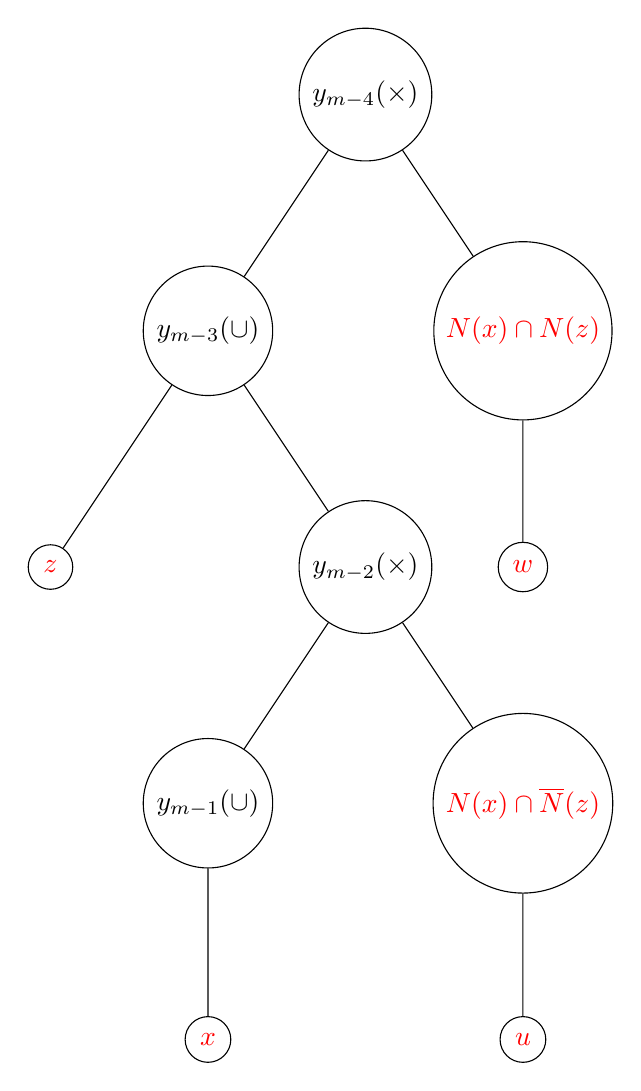
\begin{tikzpicture}[every node/.style={circle,draw,minimum size=5mm},level distance=3cm,
  level 1/.style={sibling distance=4cm},
  level 2/.style={sibling distance=2cm}
  level 3/.style={sibling distance=3cm}
  ]
    
    \node {$y_{m-4}(\times)$}
        child{ node {$y_{m-3}(\cup)$}
                 child { node {\textcolor{red}{$z$} }}
                 child { node {$y_{m-2}(\times)$}
                    child { node {$y_{m-1}(\cup)$}
                         child { node {\textcolor{red}{$x$} }}
                    }
                    child { node {\textcolor{red}{$N(x) \cap \overline{N}(z)$} }
                         child { node {\textcolor{red}{$u$} }}
                    }
                 }
        }
         child { node {\textcolor{red}{$N(x) \cap N(z)$} }
                         child { node {\textcolor{red}{$w$} }}
                    }
        ;
\end{tikzpicture}
    \caption{Vertex $z$ splits the part formed by $N(x)$}
    \label{fig:Vertex $z$ splits the part formed by $N(x)$}
\end{figure} 

First, let us prove a simpler version of the statement.

\begin{theorem}[Lemma 16 in \cite{HABIB2005183}]
    Let x be a vertex $x \notin H$ for a part H. Let $y$ and $z$ be two vertices of cograph such that $y \in N(x)$ and $z \in \bar{N}(x)$ 
    and let $P$ be a partition thinner than $\{\bar{N}(x),\{x\} ,N(x) \}$ such that there is a factorizing permutation compatible with $P$. Moreover,
    \begin{itemize}
        \item If $y$ splits a part $H \subseteq \bar{N}(x)$ then there is a factorizing permutation compatible with $P_1$ that is obtained from $P$ by refining
        $H$ into $\{  H \cap \bar{N}(y), H \cap N(y) \}$.
        \item If $z$ splits a part $H \subseteq N(x)$ then there is a factorizing permutation compatible with $P_1$ that is obtained from $P$ by refining
        $H$ into $\{  H \cap \bar{N}(z), H \cap N(z) \}$.
    \end{itemize}
    \label{General case for the Rule 2}
\end{theorem}




\begin{proof}
Let us prove only the second statement, as the first one can be done similarly.

Let $T$ be a planar representation of the cotree such that the corresponding factorizing permutation is compatible with the partition $P$.  Vertex $z$ separates part $H$. Therefore, there is a vertex $w \in H$ such that $w$ and $z$ are adjacent, and there is a vertex $u \in H$ such that $z$ and $u$ are not adjacent. Then, using \Cref{Ancestors remark}, we obtain the following facts:
\begin{enumerate}
    \item LCA$(x,u)$ is a descendant of LCA$(x,z)$.
    \item LCA$(x,z)$ is a descendant of LCA$(z,w)$.
    \item LCA$(w,z)$  $=$  LCA$(x,w)$.
    \item LCA$(x,w)$ is a series node.
    \item LCA$(x,u)$ is a series node.
    \item LCA$(x,z)$ is a parallel node.
\end{enumerate}
Thus $z$ and any vertex $v \in H$ are non-adjacent if and only if LCA$(v,z)$ $=$ LCA$(x,z)$. An example of a possible cotree is shown in \Cref{fig:Vertex $z$ splits the part formed by $N(x)$}. From the theorem statement, we know that the factorizing permutation corresponding to the cotree is thinner than partition $\{\bar{N}(x),\{x\} ,N(x) \}$. Therefore, the depth-first search visits vertex $x$ before all vertices in set $N(x)$ and after all vertices in set $\bar{N}(x)$.
Then, a left-to-right depth-first search visits all vertices in set $N(x) \cap \bar{N}(z)$ before any vertex in set $N(x) \cap N(z)$. 

Suppose the opposite that the depth-first search visited $w \in N(x) \cap N(z)$ first, then vertex $u \in N(x) \cap \bar{N}(z)$. Then the order of visiting the vertices is as follows: $z, x, w, u$. Let the least common ancestor of vertices $w$ and $x$ be vertex $y_{m-4}$, and $x$ be a descendant of vertex $y_{m-3}$, which is a child of vertex $y_{m-4}$. Since vertex $x$ is visited before vertex $w$, it follows that vertex 
$w$ is a descendant of a more right child of vertex $y_{m-4}$. 
In a left-to-right depth-first search, all vertices in the subtree $T_{y_{m-3}}$ must be visited before visiting vertex $w$. Vertex $u$ belongs to  the subtree $T_{y_{m-3}}$ so this leads to a contradiction.

Therefore, the factorizing permutation corresponding to cotree $T$ is compatible with partition obtained from $P$ by refining $H$ into $\{  H \cap \bar{N}(z), H \cap N(z) \}$.


\end{proof}

The general idea is as follows: in the algorithm, we always use Rule 1 at least once before using Rule 2. Other relationship options between part $H$ and vertex $x$ are proven similarly. Therefore, if a factorizing permutation compatible with partition $P$ existed before using Rule 2, then a factorizing permutation compatible with the partition $P_1$ obtained after using Rule 2 also exists.

\subsection{Pseudocode}
The algorithm is based on Algorithm 2 from \cite{HABIB2005183}.
Its idea for constructing a factorizing permutation is as follows: initially, the partition consists of one part. We use rules to increase the number of parts. And finally, when the number of parts becomes $|V|$, the algorithm stops.

The algorithm works in stages. At the beginning of each stage, a new vertex is chosen as the origin. Next, Rule 1 is applied to it. Then, as long as there is a part of the partition for which a pivot has not been chosen yet, we select any element of this part as the pivot and use it as a splitter for each other part of the partition.

\begin{minted}[
frame=lines,
framesep=2mm,
baselinestretch=1.2,
fontsize=\footnotesize,
linenos
]{c++}
recognition(graph G) {
     vector<parts> H;
     vector<parts> unusedParts;
     vector<nodes> N;
     H.push({V});
     Choose a random vertex of the graph as the origin
     while (|H| < |N|){
        if (H[origin].size() > 1) {
            Rule_1(origin);
            unusedParts.push(N(origin));
            unusedParts.push(origin.part / N(origin) / origin);
        }
        while (!unusedParts.empty()) {
            P = unusedParts[0];
            Choose a random vertex y of P as the pivot
            Rule_2(y);
            Mark P as used.
            for (p : newParts){
                if (The part p has no pivot){
                    unusedParts.push(p);
                }
            }
            unusedParts.erase(P);
        }  
        Let l and r be the pivots of the nearest non-singleton parts to the vertex origin 
        respectively, on the left and right sides.
        if ({l,r} belongs to the E) {
            origin = l;
        }
        else {
            origin = r;
        }
     }
}

Rule_1(node x) {
    H.erase(x.Part)
    H.push(origin.part - N(origin) - origin);
    H.push(origin);
    H.push(N(x)); 
}

Rule_2(node x) {
    for (p : H) {
        if (p != x.part) {
            if (N(x) strictly intersects p) {
                 part A = intersection of N(x) and p;
                 H.push(A);
                 H.push(p/A);
                 H.erase(p)
            }          
        }
    }
}
\end{minted}
\subsection{Correctness of the algorithm}

\begin{theorem}
    The algorithm terminates on any graph.
\end{theorem}

\begin{proof}
A part of the partition cannot be empty. Therefore, there cannot be more than $|V|$ parts in the partition.
Each use of Rule 1 increases the number of parts by at least 1.
Each use of Rule 2 increases the number of used parts in the partition. When all parts of the partition are used, Rule 1 is applied again.
Therefore, the number of parts increases after $|V|+1$ operations. Consequently, the algorithm executes a finite number of steps.
\end{proof}
\begin{invariant}
    Let $P$ be the current partition with origin $X \in V$. If $G$ is a cograph, then there is a factorizing permutation compatible $P$.
\end{invariant}

\begin{proof}
Let us prove the invariant by using induction on the number of used rules.

\begin{description}
    \item [Base Case] In the first step of the algorithm, we use Rule 1 to the partition consisting of one part containing all the vertices. The existence of a factorizing permutation after this refining is proven in \Cref{Starting case for the Rule 1}.
    \item [Inductive Step] Assume $P_i$ is the partition obtained after used $i$ rules with origin $x_i$. If $G$ is a cograph, there is a factorizing permutation compatible with $P_i$. If in the next step we use Rule 1 for vertex $v$, then for each vertex $w$ such that LCA$(x_1,w)$ is a descendant of LCA$(x_1,v)$ $H_w=\{w\}$. This is based on the case where we change the origin. We always choose the nearest vertex to the previous origin such that its part is not a singleton to be the next origin.

    The existence of a factorizing permutation after this refining is proven in \Cref{General case for the Rule 1}. If in the last step we used Rule 2, then the existence of a factorizing permutation after this refining is proven in \Cref{General case for the Rule 2} or can be proven similarly.
\end{description}


\end{proof}

\begin{theorem}[Theorem 20 in \cite{HABIB2005183}]
Algorithm  computes a factorizing permutation if the input graph is a cograph.
\end{theorem}

\begin{proof}
When any part is a singleton part, from the invariant follows that a factorizing permutation exists. Therefore the partition $P$ is a factorizing permutation.
\end{proof}

\subsection{Implementation details of the algorithm}
In this section, one of the variants of the linear implementation of the algorithm is described. We store the vertices of the graph and the parts of the partition as two doubly linked lists of structures.


Each part stores its first element, its last element, the number of elements, and its pivot (if it has one). Each element stores the part it belongs to and the next and previous element in its part.


The implementation of Rule 1 is simple. For each neighbor of vertex $x$, we check whether it is in the same part as vertex $x$.

\begin{minted}[
frame=lines,
framesep=2mm,
baselinestretch=1.2,
fontsize=\footnotesize,
linenos
]{c++}
Rule_1(node x){
   part newPart;
   for (y : N(x)) {
        if (y.part == x.part) {
            newPart.move(y);
        }
   }
   if (newPart.size() > 0) {
        H.push(newPart);
        x.part.next = newPart;
   }
   if (x.size() != 1) {
        part newPart1;
        newPart1.move(y);
        H.push(newPart1);
        x.part.next = newPart1;
   }
}
\end{minted}

From all the neighbors of $x$ that are in the same part as $x$, we create a new part. This new part is placed immediately after the part containing $x$. If there are any vertices in the part containing $x$, we split this part into two parts: the right part consists of vertex $x$, and the left part consists of all other vertices. In this way, we turn one part into 2 or 3 parts and use 
$O(|N(x))|)$ operations.

Now, let us show how to implement Rule 2 in linear time. First, for each part that contains a vertex that is a neighbor of vertex $x$ and is not equal to $x.part$, we count how many vertices in this part are neighbors of $x$.
Next, for each part that strictly intersects $N(x)$, we create a new part to the right of it. In the next loop, we move the elements into the new part.
In the final loop, we clear all the values.


\begin{minted}[
frame=lines,
framesep=2mm,
baselinestretch=1.2,
fontsize=\footnotesize,
linenos
]{c++}

Rule_2(node x) {
   for (y : N(x)) {
        y.part.amount++
   }
   for (y : N(x)) {
        if (0 < y.part.amount < y.part.size() && !y.part.part_is_created){
            part newPart_y;
            H.push(newPart_y);
            y.part.next = newPart_y;
            y.part.part_is_created = true;
        }
   }
   for (y : N(x)) {
        if(y.part.part_is_created){
            y.part.next.move(y);
        }
   }
   for (y : N(x)) {
        y.part.previous.amount = 0;
        y.part.part_is_created = false;
   } 
}
\end{minted}

The total time of Rule 2 for vertex $x$ is $O(|N(x)|)$.
\label{Implementation}

\subsection{Running time of the algorithm}

\begin{theorem}
    Rule 1 cannot be used to vertex $x$ more than once.
\end{theorem}
\begin{proof}
After using the rule to vertex $x$, the part $H_x$ becomes equal to $\{x\}$. Rule 1 is not applied to elements from singleton parts.
\end{proof}

\begin{theorem}
    Rule 2 cannot be applied to vertex $x$ as a pivot more than once.
\end{theorem}

\begin{proof}
After applying Rule 2, part $H_x$ becomes used and remains used until the end of the algorithm. Rule 2 is not applied to the pivot if its part is already used.
\end{proof}

\begin{theorem}[Theorem 24 in \cite{HABIB2005183}]
    The algorithm terminates in $O(n+m)$ time for any graph.
    \label{Running time of the factorizing permutation construction algorithm}
\end{theorem}

\begin{proof}
As proven in the \Cref{Implementation}, the time complexity of applying the rule to element $x$ is 
$O(|N(x)|)$. Each rule was applied to each vertex at most once. Therefore, the total time of the algorithm is at most $\sum\limits_{x \in V} 2 \cdot O(N(x)) = O(n+m)$. 

\end{proof}

\section{Permutation test}

\subsection{Idea}
We use the definition of a cograph from \Cref{Fundamental theorem}. A graph is called a cograph if and only if for each of its non-trivial subgraphs, there are two twin vertices. In this case, it is easy to prove that a graph is a cograph if and only if there is a twin-elimination ordering of its vertexs.
\begin{definition}[Twin-elimination ordering \cite{HABIB2005183}]
   A vertex permutation $\sigma$ is a twin-elimination ordering if and only if $\sigma=x_1,\dots,x_n$ such that for any vertex $x_i$ there are $j,i<j$ such that $x_i$ and $x_j$ are either true twins or false twins in graph $G_i=G[ \{x_i,x_{i+1},\dots,x_{n-1}\} ]$.
\end{definition}
\begin{proof}
If a twin-elimination ordering exists, then a cotree can be constructed for the graph. Thus, the graph is a cograph. More details on this can be found in \Cref{Cotree construction}.

On the other hand if the graph is a cograph, then such two twin vertices 
always exist. The proof of this follows from \Cref{Theorem on twins in the cograph}. Therefore, for any $G_i$, there is a respective $x_i$.
\end{proof}


In the permutation test algorithm, we attempt to construct a twin-elimination ordering using its vertices of permutation. If it is successful, it indicates that the permutation corresponds that graph is a cograph. Otherwise, the original graph is not a cograph.


 We construct the twin-elimination ordering from left to right. Each time when we find a suitable vertex in the obtained permutation, we remove it. Then, we have successfully constructed the twin-elimination ordering if and only if there is exactly one number left in the permutation at the end of the algorithm.
\subsection{Pseudocode}

The algorithm is based on Algorithm 5 from \cite{HABIB2005183}.

Initially, the main vertex is the first vertex in the permutation. At each step, we check if the main vertex is a twin with any of its neighbors. If it is, we remove the left vertex of this pair. If we have not removed the vertex or if the main vertex is removed, then the next main vertex is the right neighbor of the previous main vertex.

The algorithm stops when there are no more vertices to be designated as the main vertex. In other words, it happens when the rightest vertex of the permutation has been the main vertex. 

For an easier implementation, we add non-existent vertices to the beginning and to the end of the permutation. No vertex is a twin for these two added vertices. Then, the graph is a cograph if and only if, after the algorithm stops, there are exactly 3 vertices in the permutation.
\begin{minted}[
frame=lines,
framesep=2mm,
baselinestretch=1.2,
fontsize=\footnotesize,
linenos
]{c++}

Permutation test(x permutation of the vertex) {
    x[0] and x[n+1] added vertices
    mainVertex = x[1];
    while (mainVertex != x[n+1]) {
        if (mainVertex and mainVertex.previous are twins) {
            erase(mainVertex.previous);
        }
        else{
            if (mainVertex and mainVertex.next are twins) {
                mainVertex = mainVertex.next;
                erase(mainVertex.previous);
            }
            else{
                mainVertex = mainVertex.next;
            }
        }
    }
}
\end{minted}
\subsection{Constructing the cotree}
\label{Cotree construction}
\label{Constructing the cotree}
\begin{theorem}[\cite{HABIB2005183}]
    If two vertices are true (false) twins in a cograph, it is if and only if they are siblings in the cotree and their parent is a series (respective parallel) node.
    \label{Theorem on twins in the cograph}
\end{theorem}
\begin{proof}
Assume the opposite: let vertices $x$ and $y$ be true twins, but their lowest common ancestor is a parallel node. Then, by \Cref{Ancestors remark}, they are not neighbors; thus, sets $N(x) \cup \{x\}$ and $N(y) \cup \{y\}$ are not equal. Contradiction.
Assume vertices $x$ and $y$ are true twins, and their LCA is a series node, but the vertices are not siblings. Then, there is a vertex $z$ in the cograph such that the LCA $(x,z)$ is a descendant of the LCA$(x,y)$, and LCA$(x,z)$ is a parallel node. Then, vertices $x$ and $z$ are not neighbors, and vertices $y$ and $z$ are neighbors. Contradiction.
\end{proof}

Let us demonstrate an algorithm to construct a cotree from a cograph's twin-elimination ordering in linear time.

Let the twin-elimination ordering be denoted as $t=(t_1, \dots, t_n)$. At each step, the algorithm adds the rightest unprocessed vertex of the ordering to the cograph. The cotree obtained after adding vertex $t_i$ is called $T_i$.

Initially, the cotree is only the vertex  $t_{|V|-1}$. At each subsequent step, we add vertex $t_i$. We know it is a twin of some other leaf $t_j$ in the constructed cotree. We create a new internal vertex $w$ that is parallel if 
$t_i$ and $t_j$ are false twins, or series if they are true twins. To form 
$T_i$, we replace vertex $t_j$ with $w$ in $T_{i+1}$ and make $t_i$ and $t_j$ children of $w$. This replacement ensures that the LCA for each pair of leaves in $T_{i+1}$ remains unchanged, maintaining the correctness of the cotree.

Note that the resulting cotree is binary but may not always have adjacent internal nodes of different types. If a canonical cotree is needed, a depth-first search can merge adjacent nodes of the same type.

\begin{minted}[
frame=lines,
framesep=2mm,
baselinestretch=1.2,
fontsize=\footnotesize,
linenos
]{c++}
Build cotree(t twin-elimination ordering) {
   for (i = |V| - 2; i >= 0; i--) {
        j = index of vertex i twin;
        node p = t[j].parent;
        node newNode;
        if (t[i] and t[j] are true twins) {
            newNode.type = series;
        }
        else {
            newNode.type = parallel;
        }
        p.addSon(newNode);
        p.eraseSon(t[j]);
        newNode.addSon(t[j]);
        newNode.addSon(t[i]);
   }
}
\end{minted}
In order the algorithm to run in linear time, it is necessary for each vertex to store with which vertex it was removed in the twin-elimination ordering construction algorithm. Then, the time necessary to find the twin $t_j$ for vertex $t_i$ is $O(1)$. 

\subsection{Correctness of the algorithm}
It is clear that if the algorithm constructs a twin-elimination ordering, then the graph is a cograph. Let us prove the correctness of the algorithm in the other direction.

\begin{invariant}[Invariant 1 in \cite{HABIB2005183}]
    At each step of the twin-elimination ordering construction algorithm, the permutation $x$ is a factorizing permutation of the vertices of the graph $G_i$.
\end{invariant}

\begin{proof}
A factorizing permutation corresponds to some planar representation of the cotree. If we remove one leaf from this planar representation of the cotree, the leaves of each subtree appear consecutively in the permutation. Consequently, the vertices of each strong module of the new graph also appear consecutively in the permutation. Thus, the new permutation remains factorizing.
\end{proof}

Let $m_i$ be the index of the vertex that was the main one at the $i$-th iteration of the while loop in the algorithm. Let $G_i$ be the induced subgraph of the permutation $t$ at the $i$-th iteration of the while loop in the algorithm.

\begin{invariant}[Invariant 2 in \cite{HABIB2005183}]
    For any $k \ge 1$, the subsequence $t_k([m_0, \dots, m_k])$ does not contain any twins vertices in $G_k$ 
\end{invariant}

\begin{proof}
We distinguish three cases:
\begin{enumerate}
    \item $m_k$ and $m_k.previous$ are twins in $G_k$. But then $m_k.previous$ is deleted from $G_k$ and $m_{k+1} = m_k$, $t_{k+1}([m_0,\dots ,m_{k+1}])$ is included in
$t_{k}([z_0,\dots ,z_k])$, and therefore invariant is trivially true.
    \item $m_k$ and $m_k.next$ are twins in $G_k$. But then $m_k$ is deleted from $G_k$ and $m_{k+1} = m_k.next$, $t_{k+1}([m_0, \dots,m_{k+1}]) = t_{k}([m_0,\dots, m_k])$,
and therefore invariant 2 is trivially true
    \item  In the last case, we move right on the circular list, and $m_{k+1} = m_k.next$, $t_{k+1}([m_0,\dots,m_{k+1}]) = t_k([m_0,\dots,m_k])$.
\end{enumerate} 
\end{proof}

If the original graph is a cograph and after the algorithm finishes there is a permutation $g$ and $g$ has more than one vertex, then the following 3 statements are true:
\begin{itemize}
    \item each vertex in $g$ was the main vertex at the same point,
    \item $g$ is a factorizing permutation,
    \item there are two vertices belonging to $g$ such that they are twins in the graph $G[g]$.
\end{itemize}

This contradicts Invariant 2. Therefore, if the graph is a cograph, the size of the permutation after the testing is always equal to 1. 
Thus, we have proved the following theorem:

\begin{theorem}
    The size of the permutation after testing is equal to 1 if and only if it is a factorizing permutation of the cograph's vertices.
\end{theorem}

\subsection{Running time of the algorithm}

It is clear that if the algorithm constructs a twin-elimination ordering, then the graph is a cograph. Let us prove the correctness of the algorithm in the other direction.

\begin{theorem}
    The permutation algorithm terminates in $O(n+m)$ time for any graph.
    \label{Running time of the permutation verification algorithm}
\end{theorem}

\begin{proof}
Each vertex is the main vertex in no more than 2 twin checks. The twin check for vertices x and y takes a $\min\{|N(x)|,|N(y)|\} $ time. To get this, it is necessary to store the vertexs edges in sorted order. Then, the total time of the testing algorithm is no more than $\sum\limits_{u \in V} 2 \cdot O(|N(x)|) = O(n+m)$.
\end{proof}

\begin{theorem}
    The recognition algorithm terminates in $O(n+m)$ time for any graph.
\end{theorem}
\begin{proof}
By \Cref{Running time of the factorizing permutation construction algorithm} and \Cref{Running time of the permutation verification algorithm} both parts of the algorithm run in linear time; therefore, the entire algorithm runs in linear time.
\end{proof}
\chapter{Algorithmic properties of cographs}
\label{Properties}
\section{Idea}
The algorithms are inspired by \cite{CORNEIL1981163}.
Having a cotree corresponding to the given cograph, we can compute various graph parameters using dynamic programming, e. g; treewidth,  maximum clique or similar parameters. Typically, we calculate them in a bottom-up manner using e.g depth-first search on the cotree in binary form. Initially, the parameter value is computed for all descendants of a vertex, and then for the vertex itself. For recalculation, we use the fact that knowing the type of vertex (parallel or series), we know which edges exist in the cograph between the leaves of different subtrees of the cotree.

\section{Maximum clique}

The idea of calculating the maximum clique is as follows:
\begin{itemize}
    \item If the cograph consists of only one vertex, then the size of the maximum clique is 1.
    \item If If the root of the cotree is a parallel vertex, then the graph $G=G_1 \cup G_2 \cup \dots \cup G_k$. Hence, the maximum clique of the cograph is the largest maximum clique among the graphs $G_1 , \dots , G_k$. Therefore, the maximum clique of the graph equals the maximum clique among all the children of the root.
    \item If the root of the cotree is a series vertex, then the graph $G=G_1 \times G_2 \times \dots \times G_k$. Consequently, all the leaves from different subtrees of the root's children are adjacent in the cograph. Then, the set of vertices $v_1, \dots , v_f$ forms a clique if and only if for every pair of vertices $v_i$ and $v_j$, either $v_i$ and $v_j$ are descendants of different children of the root, or $v_i$ and $v_j$ are neighbors. Therefore, the maximum clique of the graph equals the sum of the maximum cliques of its children.

    Such a formula can be computed in linear time using a depth-first search.

    The first depth-first search calculates the size of the maximum clique for each cograph corresponding to a subtree of the cotree.
The second depth-first search finds any set of vertices in the graph that form a maximum clique.
\end{itemize}

\begin{minted}[
frame=lines,
framesep=2mm,
baselinestretch=1.2,
fontsize=\footnotesize,
linenos
]{c++}

Maximum clique(cotree T) {
   Maximum subtree clique size(tree root);
   Add maximum subtree clique(tree root);
}
Maximum subtree clique size(node x) {
    if (x.type == leaf) {
        return 1;
    }
    if (x.type == parallel) {
        return max(Maximum subtree clique(x.leftSon), Maximum subtree clique(x.rightSon));
    }
    if (x.type == series) {
         return Maximum subtree clique size (x.leftSon) + Maximum subtree clique size(x.rightSon);
    }
    return x.subtree_clique_size;
}

Add maximum subtree clique (node x) {
    if (x.type == leaf) {
        Clique.add(x);
    }
    if (x.type == parallel) {
        if (x.leftSon.subtree_clique_size >= x.rightSon.subtree_clique_size){
            Add maximum subtree clique(x.leftSon);
        }
        else {
            Add maximum subtree clique(x.rightSon);
        }
    }
    if(x.type == series) {
        Add maximum subtree clique(x.leftSon);
        Add maximum subtree clique(x.rightSon);
    }
}

\end{minted}

\section{Graph coloring}
The coloring algorithm for a cograph use a similar scheme to the previous algorithms. We color the subtrees of the cograph using the properties of parallel and series vertices. If the graph is a parallel composition of cographs $G_1, \dots , G_k$ then the cographs $G_1, \dots ,G_k$ can be colored independently. If the graph is a series composition of cographs $G_1, \dots , G_k$ then the leaves that are descendants of different children of the root cannot have the same color. Therefore, the chromatic number of the cograph is equal to the sum of the chromatic numbers of the cographs $G_1, \dots ,G_k$. The first cograph can be colored with colors $1 \dots \chi(G_1)$ , the second cograph with colors $\chi(G_1)+1, \dots, \chi(G_1)+\chi(G_2)$ and so on.

\begin{minted}[
frame=lines,
framesep=2mm,
baselinestretch=1.2,
fontsize=\footnotesize,
linenos
]{c++}

void Graph coloring (){
    Subtree coloring(tree root, 0);
}

int Subtree coloring(node x ,number of occupied colors k){
    if (x.type == leaf) {
        x.color = k + 1;
    }
    int l = Subtree coloring(x.leftSon, k);
    if (x.type == parallel) {
       int r = Subtree coloring(x.rightSon, k);
       return max(l, r);
    }
    if (x.type == series) {
       int r = Subtree coloring(x.rightSon, l);
       return r;
    }
}
\end{minted}
\label{Max}
\section{Independent set}

The idea of finding an independent set is similar to the one presented above, since the maximum independent set is the maximum clique of the complement graph. The algorithm for finding the maximum clique was discussed in \Cref{Max}. It is sufficient to build the cotree of the complement cograph in linear time.
\begin{theorem}
If $T$ is the cotree of graph $G$ and $T'$ is the cotree of graph $G'$, where 
$T'$ is obtained from $T$ by changing the types of vertices (parallel nodes to series nodes and vice versa), then $G=\bar{G'}$.
\end{theorem}

\begin{proof}
Vertices $x$ and $y$ are neighbors in the cograph $G$ if and only if their lowest common ancestor in the cotree $T$, denoted by $w$, is a series vertex. From the definition of cotree $T'$, the vertex $w$ in cotree $T'$ is a parallel vertex. Therefore, vertices $x$ and $y$ are neighbors in cograph $G$ if and only if they are not neighbors in graph $G'$.
\end{proof}

\section{Treewidth and pathwidth}
Theorems and algorithms are taken from \cite{Sumner1974DaceyG}.

The basis of the algorithm is the theorem on the relationship between pathwidth and treewidth with parallel and series composition.
\begin{theorem} [Lemma 3.4 in \cite{Sumner1974DaceyG}]
    Let $G_1=(V_1,E_1)$, $G_2=(V_2,E_2)$ be graphs. Then the following conditions hold:
    \begin{itemize}
        \item $tw(G_1\cup G_2)= \max\{tw(G_1), tw(G_2)\}$.
        \item $pw(G_1\cup G_2)= \max\{pw(G_1), pw(G_2)\}$.
        \item $tw(G_1\times G_2)= \min\{tw(G_1) + |V_2|, tw(G_2) + |V_1|\}$.
        \item $pw(G_1\times G_2)= \min\{pw(G_1) + |V_2|, pw(G_2) + |V_1|\}$.
    \end{itemize}
    \label{Theorem on treewidth in a binary cotree}
\end{theorem}

The complete proof of \Cref{Theorem on treewidth in a binary cotree} can be found in \cite{Sumner1974DaceyG}.
 The idea of the proof is as follows. If a cograph $G$ is a parallel composition of two cographs $G_1$, $G_2$, then the tree decomposition $(I,T)$ of the graph $G$ is simply the union of the tree decompositions of graphs $G_1$ and $G_2$. $I=(I_1 \cup I_2), T=(T_1 \cup T_2)$ hence $tw(G)= \max\{(tw(G_1), tw(G_2)\}$.

 If a cograph is a series composition of cographs $G_1=(V_1,E_1)$ and $G_2=(V_2,E_2)$ and $(I_1,T_1)$ is tree decomposition of $G_1$ and $(I_2,T_2)$ is tree decomposition of $G_2$, then it is sufficient to prove the inequality in two directions:
 \begin{enumerate}
     \item $tw(G)\le \min\{tw(G_1) + |V_2|, tw(G_2) + |V_1|\}$.
     \item $tw(G)\ge \min\{tw(G_1) + |V_2|, tw(G_2) + |V_1|\}$.
 \end{enumerate}
 Let $tw(G_1) + |V_2| \le tw(G_2) + |V_1|$. Then the pair $(X_i \cup |V_2| \colon i \in I_1,T_1)$ is a tree decomposition of the cograph $G$. It holds that $\max\limits_{i \in I_1} |X_i \cup V_2| \le tw(G_1) + |V_2|$ hence $tw(G)\le \min\{tw(G_1) + |V_2|, tw(G_2) + |V_1|\}$.

The proof of the inequality in the opposite direction can be found in \cite{Sumner1974DaceyG}.
   
\begin{theorem}[Theorem 3.2 \cite{Sumner1974DaceyG}]
     For every cograph $G$, it holds that $tw(G) = pw(G)$.
\end{theorem}

\begin{proof}
    We can prove the equality of pathwidth and treewidth for every cograph using induction on the number of vertices.
    \begin{description}
        \item[Base case] For a graph consisting of a single vertex, the pathwidth and treewidth are the same and equal to 0.
        \item[Induction step] Assume that for all cographs with less than $n+1$ vertices, the pathwidth and treewidth are the same. Let $G=(V, E)$ be any cograph with $n+1$ vertices. Let $T$ be the cotree corresponding to $G$. If the root of $T$ is a parallel vertex, then there exist two cographs $G_1$ and $G_2$ such that $G=G_1 \cup G_2$. From \Cref{Theorem on treewidth in a binary cotree}, it follows that $tw(G_1 \cup G_2)= \max \{tw(G_1), tw(G_2)\}$ and $pw(G_1 \cup G_2)= \max \{pw(G_1), pw(G_2)\}$.
        However, the number of vertices in $G_1$ and $G_2$ is less than $n+1$. Therefore, $tw(G_1)=pw(G_1)$ and $tw(G_2)=pw(G_2)$. Then $tw(G)=pw(G)$. The case where the root of the cotree is a series vertex is proved similarly.
    \end{description}

\end{proof}
Next, using dynamic programming on the cotree, we find the number of vertices in the subtree of each vertex. In the following depth-first search, we find the pathwidth and treewidth for each subtree.

\begin{minted}[
frame=lines,
framesep=2mm,
baselinestretch=1.2,
fontsize=\footnotesize,
linenos
]{c++}

int Graph pathwidth(cotree T) {
   Subtree sizes(tree root);
   return Subtree pathwidth(tree root);
}

void Subtree sizes(node x) {
    if (x.type == leaf) {
        x.subtree_size = 1;
    }
    else {
        Subtree sizes(x.leftSon);
        Subtree sizes(x.rightSon);
        x.subtree_size = x.leftSon.subtree_size + x.rightSon.subtree_size
    }
}

int Subtree pathwidth(node x) {
    if (x.type == leaf){
        return 1;
    }
    if (x.type == parallel) {
        return max(Subtree pathwidth(x.leftSon), Subtree pathwidth(x.rightSon));
    }
    if (x.type == series) {
         return min(Subtree pathwidth(x.leftSon) + x.rightSon.subtree_size,
         Subtree pathwidth(x.rightSon) + x.leftSon.subtree_size);
    }
    return x.subtree_clique_size;
}

\end{minted}



\chapter{Implementation}
\label{last}
\section{Introduction}
The algorithms described above were implemented in C++. For graph operations, the NetworKit and Koala libraries were used. The code is open source and available in the Koala-NetworKit GitHub repository at 
\url{https://github.com/krzysztof-turowski/koala-networkit/pull/23}.

\section{Implementation details}
The repository contains separate classes for each type of problem, such as cograph recognition, treewidth calculation, maximum clique calculation, and so on. Below is a brief description of the files with their purposes.
\begin{itemize}
    \item \texttt{koala-networkit/include/recognition/CographRecognition.hpp}

    The main header file defining the cograph recognition class.

    \item \texttt{koala-networkit/include/recognition/cograph/Part.hpp}
    
    Header file for the class implementing the Part and Element classes used by the recognition algorithm.
    
    \item \texttt{koala-networkit/include/recognition/cograph/FactorizingPermutation.hpp}
    
    Header file for the class implementing the creation and manipulation of a factorizing permutation. For example, adding or removing parts or elements, moving elements to different parts, and so on. It is used in the factorizing permutation construction algorithm.

    \item \texttt{koala-networkit/include/recognition/cograph/Twins.hpp}
    
    Header file for the class implementing operations with twin vertices in a cograph. For example, checking if vertices are twins. It is used in the single permutation testing algorithm.

    \item \texttt{koala-networkit/include/structures/Cotree.hpp}

Header file for the class implementing operations on the cotree and its vertices.
\item \texttt{koala-networkit/include/pathwidth/CographPathwidth.hpp}

Header file for the class implementing the calculation of graph pathwidth.
\item \texttt{koala-networkit/include/coloring/CographVertexColoring.hpp}

Header file for the class that finds the graph coloring with the minimum number of colors.

\item \texttt{koala-networkit/include/independent\_set/CographIndependentSet.hpp}

Header file for the class that finds the independent set of a graph.
\item \texttt{koala-networkit/include/max\_clique/CographMaxClique.hpp}

Header file for the class that finds the maximum clique of a graph.

\item \texttt{koala-networkit/benchmark/}

Folder containing benchmarking programs to evaluate the performance of the algorithms on various graph instances.

\item \texttt{koala-networkit/test/}

Folder containing unit tests for checking correctness of the implemented algorithms.

\end{itemize}
\section{Testing}
The correctness of each algorithm was tested in two ways:
\begin{enumerate}
    \item Unit tests on all small-sized graphs, i.e.  graphs with less than $15$ vertices. 
    \item On graphs from the benchmark containing random cographs and non-cographs with less than $10^6$ vertices.
\end{enumerate}

The following iterative algorithm generates random cographs. First, create $n$ cographs, each consisting of a single vertex. At each step, select and merge two random cographs into one. Then, with a given probability $p$, replace the cograph with its complement. The algorithm stops when all cographs merge into one. This algorithm can produce any cograph with $n$ vertices. At step $i$, merge cographs $G_i^1$ and $G_i^2$. 
Let the set $B_{x,y}=\{i \colon x,y \in (G_i^1 \cup G_i^2)\}$ include all the steps in which vertices $x$ and $y$ participated in the merging. Vertices $x$ and $y$ become neighbors if and only if the number of times the complement is used during these operations is odd. The probability of this is $1-\sum\limits_{i=0}^{|B|/2} \binom{|B|}{2 \cdot i}$. This fact allows generating graphs with a specific number of edges. For example, if $p=\frac{1}{2}$, then the probability of an edge existing between any pair of vertices is $\frac{1}{2}$. This follows from the well-known fact that forall n it is true that $\sum\limits_{i=0}^{i=n} {(-1)}^i \cdot \binom{n}{i}=0$.

\section{Running time}

The explanations of the algorithm names are provided in \Cref{tab:algorithms_number}.
The algorithms were tested on several subgroups of tests. 
Each test consists of 5 random graphs generated with the same number of edges and vertices. The average runtime, in milliseconds, are presented in \Cref{tbl:algorithms} and \Cref{tbl:algorithms1}. 



\begin{table}[]
    \centering
    \begin{tabular}{ | c | p{4cm} |}
  \hline
  Id & Algorithm \\ [0.5ex] 
  \hline\hline
  $A1$ &  Cograph recognition \\
  \hline
  $A2$ &  Independent set  \\
  \hline
  $A3$ &  Max clique \\
  \hline
  $A4$ &  Pathwidth \\
  \hline
  $A5$ &  Vertex coloring \\
  \hline
  \end{tabular}
  \caption{The algorithms numbers with their identifiers}
    \label{tab:algorithms_number}
\end{table}

  
\begin{table}[ht]
\centering
\begin{tabular}{ | c | c | c |}
\hline
$n$ & $m$ & $A1$    \\ [0.6ex] 
 \hline
 $10^3$ & $5 \cdot 10^3$ & 2  \\ [0.6ex] 
\hline
 $7*10^4$ & $10^5$ & 7100  \\ [0.6ex] 
  \hline
 $10^5$ & $2 \cdot 10^6$ & 49000  \\ [0.6ex] 
 \hline
 $10^6$ & $4 \cdot 10^7$ & $17 \cdot 10^5$  \\ [0.6ex] 
 \hline
\end{tabular}

\caption{The running time of the cograph recognition algorithm}
\label{tbl:algorithms}
\end{table}


\begin{table}[ht]
\centering
\begin{tabular}{ | c | c | c | c | c | }
\hline
$n$ & $A2$ & $A3$ & $A4$ & $A5$   \\ [0.6ex]
\hline
$10^5$ & 3 & 15 & 5 & 12 \\ [0.6ex] 
\hline
$5 \cdot 10^5$ & 16 & 108 & 26 & 90 \\ [0.6ex] 
\hline
$10^6$ & 33 & 238 & 53 & 189 \\ [0.6ex] 
\hline
$4 \cdot 10^6$ & 144 & 1369 & 212 & 910 \\ [0.6ex] 
\hline
$8 \cdot 10^6$ & 292 & 3157 & 425 & 2079 \\ [0.6ex] 
\hline
$2 \cdot 10^7$ & 732 & 9584 & 1105 & 6039 \\ [0.6ex]
\hline
$5 \cdot 10^7$ & 1993 & 28287 & 2741 & 18316 \\ [0.6ex]
\hline

\end{tabular}

\caption{The running time of different algorithms on cographs}
\label{tbl:algorithms1}
\end{table}


\section{Conclusions}

It is clear that the number of edges in the graph does not affect the performance of algorithms $A2, A3, A4, A5$. This is because these algorithms do not operate on the original cograph, but only on the constructed cotree. The algorithm from \Cref{Cotree construction} always constructs a cotree with $O(n)$ edges. The \Cref{fig:milliseconds} shows that these algorithms run in linear time and, within the tested range.

\begin{figure}[h!]
  \centering
  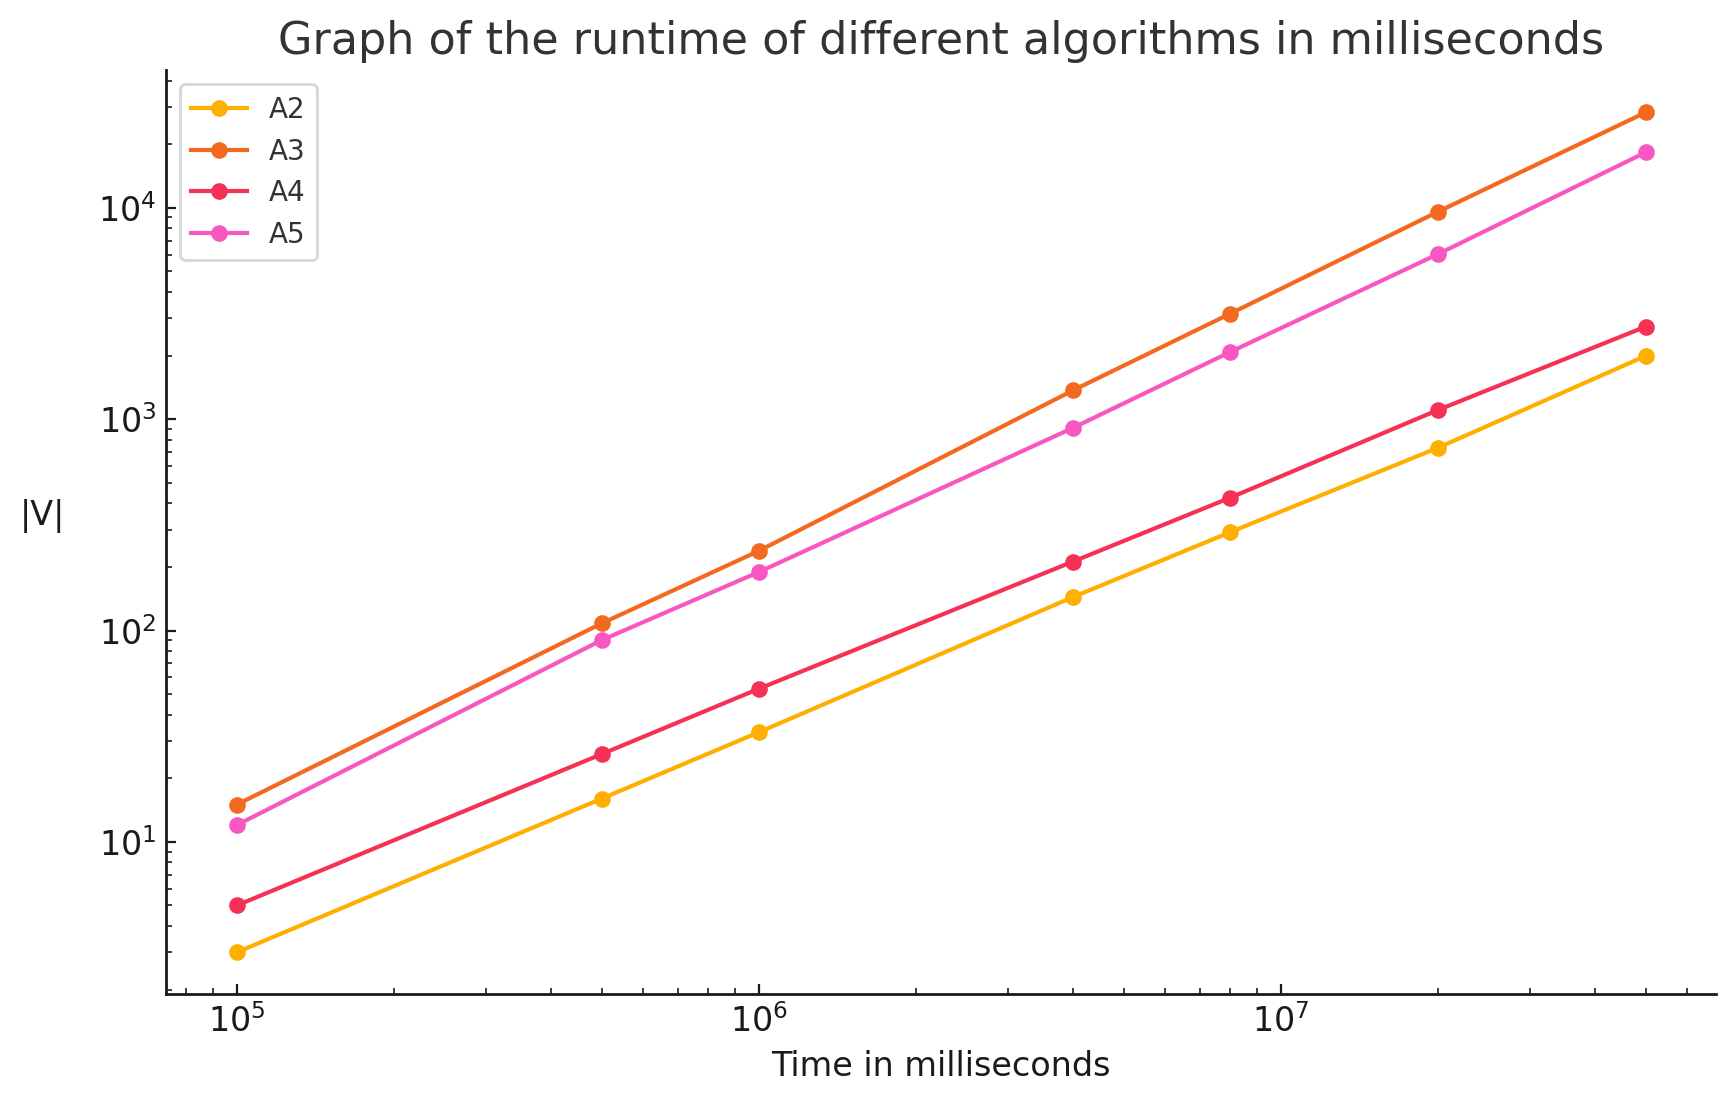
\includegraphics[width=\linewidth]{output (3).png}
  \caption{Graph of the runtime of different algorithms in milliseconds.}
  \label{fig:milliseconds}
\end{figure}


\begin{figure}[h!]
  \centering
  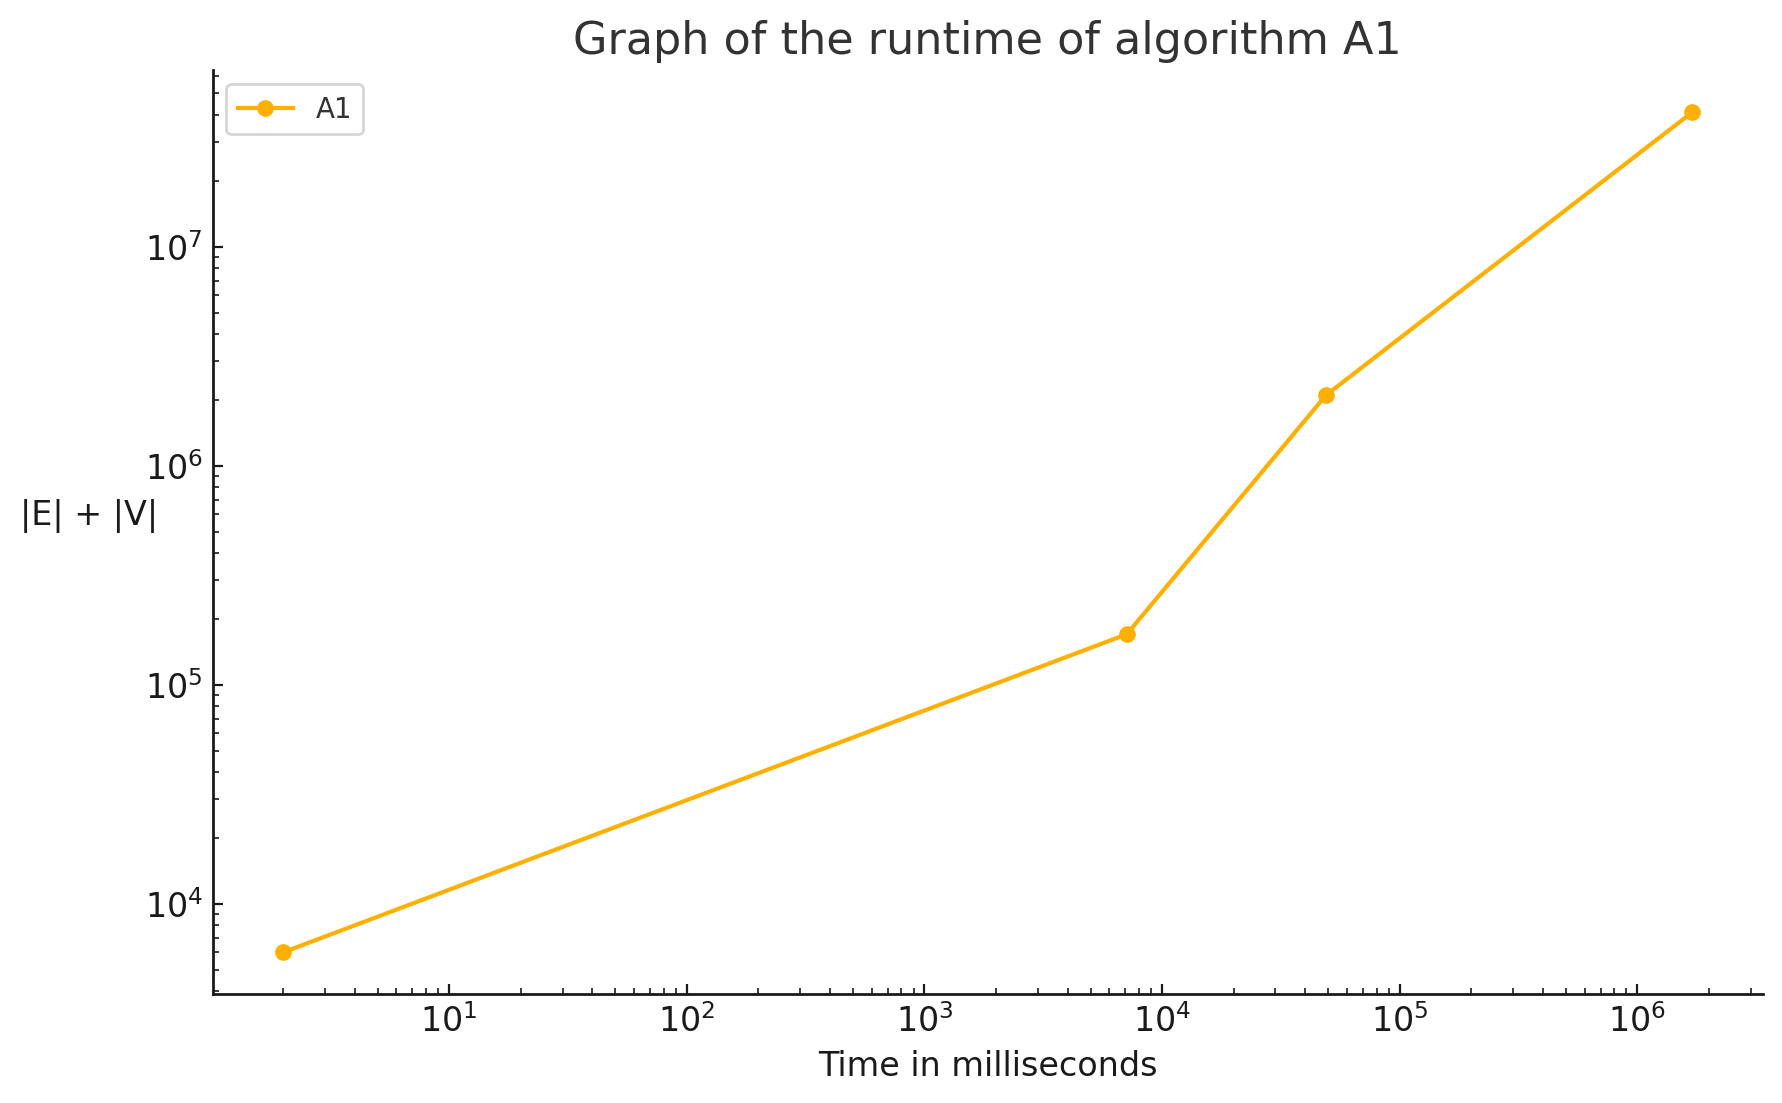
\includegraphics[width=\linewidth]{output (2).png}
  \caption{Graph of the runtime of $A1$ algorithm in milliseconds.}
  \label{fig:100milliseconds}
\end{figure}

The running time of the algorithm A1 depends on both the number of edges and the number of vertices. From the \Cref{fig:100milliseconds} and \Cref{tbl:algorithms} values, it is clear that the algorithm is linear within the tested range.
\printbibliography
\end{document}